% !TeX encoding = UTF-8
% !TeX program = pdflatex

\documentclass[a4paper]{article}
\usepackage[T1]{fontenc}
\usepackage[utf8]{inputenc}
\usepackage[english]{babel}
\usepackage{hyperref}
\usepackage{cite}
\usepackage{graphicx}
\graphicspath{{../Results/}}
\usepackage{mathtools}
\usepackage{amsfonts}
\usepackage[labelformat=empty]{caption}
\usepackage{grffile}

\title{Reproducing results of \\
	"Enhancing adversarial defense by k-WTA"}
\author{Marco Costa, Andrea Luca Antonini}

\begin{document}
	
	\maketitle
	
	\section{Introduction}
	The goal of our project is to demonstrate the reproducibility of the paper ”Enhancing Adversarial Defense by k-Winners-Take-All” (Xiao et al.) \newline
	The use of k-WTA activation is motivated for defending against gradient-based adversarial attacks. In fact, provided a labeled data item (\textbf{x},y), the attacker finds a perturbation \textbf{x'} imperceptibly similar to \textbf{x} but misleading enough to cause the network to output a label different from y. The most effective way to find such a perturbation, i.e. adversarial example, is by exploiting the gradient information of the network w.r.t. its input \textbf{x}. \newline
	k-WTA activation function takes as input the entire output of a layer, retains its \textit{k} largest values and deactivates all others to zero. If we use $f(\textbf{x};\textbf{w})$ to denote a k-WTA network taking an input \textbf{x} and parameterized by weights \textbf{w}, then the gradient $\nabla_{\textbf{x}}f(\textbf{x};\textbf{w})$ at certain \textbf{x} is undefined. Therefore, $f(\textbf{x};\textbf{w})$ is C$^0$ discontinous. The discontinuities in the activation function also renders $f(\textbf{x};\textbf{w})$ discontinous w.r.t. \textbf{w}, but these discontinuities are rather sparse in the space of \textbf{w}, thus the network can be trained succesfully. \newline
	Formally, k-WTA retains the \textit{k} largest values of a $N$x$1$ input vector and sets all others to be zero before feeding the vector to the next network layer:
	
	\begin{equation}
	\phi_{k}(\textbf{y})_{j} = 
	\begin{cases*}
	y_{j}\textrm{, if }y_{j} \in\{\textrm{\textit{k} largest elements of \textbf{y}}\} \\
	0 \textrm{, otherwise}
	\end{cases*}
	\end{equation}
	where $\phi_{k}: \mathbb{R}^{N} \rightarrow \mathbb{R}^{N}$ is the k-WTA function (parameterized by an integer \textit{k}), \textbf{y} $\in \mathbb{R}^{N}$ is the input to the activation, and $\phi_{k}(\textbf{y})_{j}$ denotes the j-th element of the output $\phi_{k}(\textbf{y})$.\\
	Instead of specifying \textit{k}, it's possible to introduce a parameter $\gamma \in \{0,1\}$ called \emph{sparsity ratio}. If a layer has an output dimension $N$, then its k-WTA activation has  $k = \lfloor\gamma \cdot N\rfloor$. Even though the sparsity ratio can be set differently for different layers, in practice there is no gain from introducing such a variation, so we use a fixed $\gamma$.\\
	In a Convolutional Neural Network (CNN), the output of a layer is a C x H x W tensor: in this case we will treat the tensor as a C $\cdot$ H $\cdot$ W x 1 vector input to the k-WTA activation function.\\
	The runtime of computing a k-WTA activation is asymptotically $O(N)$, because finding \textit{k} largest value in a list corresponds to finding the k-th largest value, which has $O(N)$ complexity.\\
	Concerning the training of k-WTA networks, when the sparsity ratio $\gamma$ is relatively small ($\le 0.2$), the network training converges slowly. In fact, a smaller $\gamma$ activates fewer neurons, effectively reducing more of the layer width and, therefore, the network size. Nevertheless, it is preferable to use a smaller $\gamma$ because it usually leads to better robustness against finding adversarial examples.\\
	Theoretically speaking, consider one layer outputting values \textbf{x}, passed through  a k-WTA activation, and followed by the next layer whose linear weight matrix is
	W. We define the k-WTA \emph{activation pattern} under the input \textbf{x} as:
	\begin{center}
		$\mathcal{A}(\textbf{x}) := \{i \in [l]$ | $x_{i}$ is one of the \textit{k} largest values in \textbf{x}$\} \subseteq [l]$
	\end{center}
	where we use $[l]$ to indicate integer set $\{1,...,l\}$.\\
	Even an infinitesimal perturbation of \textbf{x} can change $\mathcal{A}(\textbf{x})$: some element $i$ is removed from $\mathcal{A}(\textbf{x})$, while another element $j$ is added in. Corresponding to this change, in the evaluation of $W\phi_{k}(\textbf{x})$, the contribution of $W$'s column vector $W_{i}$ is useless, while another column vector $W_{j}$ suddenly takes effect. It's this change that makes the result of $W\phi_{k}(\textbf{x})$ $C^0$ discontinous.\\
	Once $W$ is determined, the discontinuity jump depends on the value of $x_i$ and $x_j$, that are respectively the input value that does no more affect the result and the new value that actually has effect. The smaller $\gamma$ is, the larger the discontinuity jump will be: for this reason, it is recommended to use a smaller $\gamma$, that will make the search of adversarial examples harder.\\
	If the activation patterns of all layers are fixed, then f(\textbf{x}) is a linear function, but when the activation pattern changes, f(\textbf{x}) switches from one linear function to another linear function. Over the entire space of \textbf{x}, f(\textbf{x}) is \emph{piecewise linear}. The specific activation patterns of all layers define a specific linear piece of the function, i.e. a \emph{linear region}: in k-WTA, these linear regions are disconnected.\\
	If the linear regions are densely distributed, a small perturbation $\Delta\textbf{x}$ from any data point will likely cross the boundary of the linear region where \textbf{x} is. Whenever boundary crossing occurs, the gradient becomes undefined.\\
	The rationale behind k-WTA activation is to destroy network gradients, that are information needed in \emph{white box attacks}.\\
	k-WTA is able to universally improve the white-box robustness, regardless of the training method. The k-WTA robustness under \emph{black box attacks} is not always significantly better than other activation function networks (e.g. ReLU).
	
	\section{Approach}
	The core of our approach is to substitute the most commonly used activation functions (e.g. ReLU) with k-WTA and measure their performance and robustness to adversarial attacks.
	The idea is to compare the performance of the models with k-WTA with those who have a most common ReLU.
	In order to do this, we used two different networks, i.e. \textbf{\textit{ResNet}} and \textbf{\textit{AlexNet}}, trained on different datasets, i.e. \textbf{\textit{CIFAR-10}} and \textbf{\textit{SVHN}}.\\
	By examining the resulting robustness of the trained models, we wanted to confirm the effectiveness of the method.
	
	\section{Experiments}
	\subsection{Frameworks and Data}
	All the experiments have been done with Pytorch deep learning framework, using GPU acceleration for the execution of the experiments.\\
	As said before, we considered ResNet and AlexNet models using the standard implementations of ResNet18 and AlexNet architecture from the Torchvision package. We used these networks in two ways. First, using the pre-trained models on ImageNet dataset, modifiying the final layer to output 10 features and fine-tuned the models on CIFAR-10 and SVHN dataset. Second, training the networks from scratch, directly on CIFAR-10 and SVHN datasets.
	
	\subsection{Training models}
	In order to train the models we proceeded as follows: \\
	For networks that use the \textit{ReLU} activation function, we have simply traied them with 80 epochs for models trained from scratch and 10 epochs for pre-trained models. For networks that use the \textit{k-WTA} activation function, instead, we replaced the \textit{ReLU} activation layer with \textit{k-WTA} using two sparsity ratio, first $\gamma = 0.2$ and then $\gamma = 0.1$, using the same training scheme seen before (80 epochs for models trained from scratch, 10 for pre-trained models). \\
	The authors of the paper, instead, used a different approach. For k-WTA networks with a sparsity ratio $\gamma = 0.1$, they trained them incrementally, starting with $\gamma = 0.2$ for 50 epochs with SGD and then decreasing $\gamma$ by $0.005$ every 2 epochs until it reached $0.1$. \\
	We noticed that, obvoiusly, training the models from scratch is much more expensive in terms of time than training pre-trained models.\\
	Our training dataset was preprocessed with random cropping and random horizontal flipping. Finally, we additionally scaled up images to 224x224 since the Torchvision pre-trained model architectures expect this input dimensionality.\\
	We used a batch size of 64 in the data loaders.\\
	All of our models used the Cross Entropy loss function and were trained with Stochastic Gradient Descent using	a learning rate of $0.01$ for pre-trained models, while for the others learning rate is set to $0.1$ for the first 50 epochs, while for the remaining 30 is manually changed to 0.01. \\ Moreover, we inserted a momentum of $0.9$, and in order to avoid exploding gradients we also used gradient clipping with a max norm of $0.5$
	
	\subsection{Robustness to Adversarial attacks}
	k-WTA activation function, as explained in the introduction, is wanted to be a defence against attacks that exploit the gradient of the network. In order to neutralize these attacks, k-WTA, thanks to its densely piecewise continous nature, destroys network gradients and, therefore, represents a counterpoison to the venom of attacks, specially white box attacks. Our goal is to test the effective robustness to adversarial attacks of the models using k-WTA activation function, comparing the results with models using ReLU activation function. To achieve this, we tested the various models ((Resnet | AlexNet) + (k-WTA | ReLU)) under two kind of attacks, namely Projected Gradient Descent (\textbf{\textit{PGD}}) and \textbf{\textit{Deepfool}}. Both the attacks are run using the Foolbox third-party toolkit.\\
	We used a perturbation $\epsilon = 0.031$ in the case of CIFAR-10 dataset, while in the case of SVHN dataset $\epsilon = 0.047$. PGD attack is carried on for 40 steps, with random starting and relative step size of $0.003$. Instead, Deepfool attack is run for 20 steps with a candidate sub-sampling parameter of 10. The attacks were executed for 20 mini-batches with batch size 64.
	
	\subsection{Results}
	In \textit{Table 1} and \textit{Table 2} we show the results for training an AlexNet network on SVHN and CIFAR-10 respectively, using ReLU, k-WTA with $\gamma = 0.2$ and k-WTA with $\gamma = 0.1$. The value $A_{std}$ indicates the standard test accuracy, while the other two columns show the robustness accuracy under PGD and Deepfool attacks. \textit{Table 3} and \textit{Table 4} illustrates the results with the networks with same characteristics, but with the difference that they are pre-trained.
	A series of graphics representing \emph{accuracy}, \emph{loss} and \emph{error} of the various experiments can be found in \emph{Appendix A}.
	\begin{table}[!htbp]
		\begin{tabular}{|p{0.2\textwidth}|p{0.2\textwidth}|p{0.2\textwidth}|p{0.2\textwidth}|}
			\hline
			Activation	& $A_{std}$	&	PGD	&	Deepfool	\\
			\hline
			ReLU		&$19.59\%$&$20.31\%$&$16.25\%$	\\
			\hline
			k-WTA-0.2	&$94.65\%$&$26.88\%$&$1.25\%$	\\
			\hline
			k-WTA-0.1	&$19.59\%$&$20.94\%$&$16.88\%$	\\
			\hline
		\end{tabular}
		\caption{Table 1: AlexNet experiment results with SVHN}\label{alexnetSVHN}
	\end{table}
	\begin{table}[!htbp]
		\begin{tabular}{|p{0.2\textwidth}|p{0.2\textwidth}|p{0.2\textwidth}|p{0.2\textwidth}|}
			\hline
			Activation	& $A_{std}$	&	PGD	&	Deepfool	\\
			\hline
			ReLU		&$86.66\%$&$48.44\%$&$0.00\%$	\\
			\hline
			k-WTA-0.2	&$87.22\%$&$59.38\%$&$0.00\%$	\\
			\hline
			k-WTA-0.1	&$88.98\%$&$52.19\%$&$0.00\%$	\\
			\hline
		\end{tabular}
		\caption{Table 2: AlexNet experiment results with CIFAR-10}\label{alexnetCIFAR10}
	\end{table}
	\begin{table}[!htbp]
		\begin{tabular}{|p{0.2\textwidth}|p{0.2\textwidth}|p{0.2\textwidth}|p{0.2\textwidth}|}
			\hline
			Activation	& $A_{std}$	&	PGD	&	Deepfool	\\
			\hline
			ReLU		&$92.09\%$&$20.62\%$&$0.00\%$	\\
			\hline
			k-WTA-0.2	&$91.76\%$&$20.62\%$&$0.00\%$	\\
			\hline
			k-WTA-0.1	&$91.71\%$&$30.94\%$&$0.00\%$	\\
			\hline
		\end{tabular}
		\caption{Table 3: Pre-trained AlexNet experiment results with SVHN}\label{pre-alexnetSVHN}
	\end{table}
	\begin{table}[!htbp]
		\begin{tabular}{|p{0.2\textwidth}|p{0.2\textwidth}|p{0.2\textwidth}|p{0.2\textwidth}|}
			\hline
			Activation	& $A_{std}$	&	PGD	&	Deepfool	\\
			\hline
			ReLU		&$87.95\%$&$5.00\%$&$0.00\%$	\\
			\hline
			k-WTA-0.2	&$87.23\%$&$15.31\%$&$0.00\%$	\\
			\hline
			k-WTA-0.1	&$83.67\%$&$36.56\%$&$0.00\%$	\\
			\hline
		\end{tabular}
		\caption{Table 4: Pre-trained AlexNet experiment results with CIFAR-10}\label{pre-alexnetCIFAR10}
	\end{table}\\
	Then, we show the experiment results for training using network ResNet18, with SVHN dataset (\textit{Table 5}) and CIFAR-10 dataset (\textit{Table 6}) on ReLU, k-WTA-0.2 and k-WTA-0.1.
	\begin{table}[!htbp]
		\begin{tabular}{|p{0.2\textwidth}|p{0.2\textwidth}|p{0.2\textwidth}|p{0.2\textwidth}|}
			\hline
			Activation	& $A_{std}$	&	PGD	&	Deepfool	\\
			\hline
			ReLU		&$94.91\%$&$28.44\%$&$0.00\%$	\\
			\hline
			k-WTA-0.2	&$95.82\%$&$70.31\%$&$13.12\%$	\\
			\hline
			k-WTA-0.1	&$95.02\%$&$77.81\%$&$33.12\%$	\\
			\hline
		\end{tabular}
		\caption{Table 5: ResNet18 experiment results with SVHN}\label{resnetSVHN}
	\end{table}
	\begin{table}[!htbp]
		\begin{tabular}{|p{0.2\textwidth}|p{0.2\textwidth}|p{0.2\textwidth}|p{0.2\textwidth}|}
			\hline
			Activation	& $A_{std}$	&	PGD	&	Deepfool	\\
			\hline
			ReLU		&$92.29\%$&$28.44\%$&$0.00\%$	\\
			\hline
			k-WTA-0.2	&$85.20\%$&$68.75\%$&$14.38\%$	\\
			\hline
			k-WTA-0.1	&$79.90\%$&$58.44\%$&$26.56\%$	\\
			\hline
		\end{tabular}
		\caption{Table 6: ResNet18 experiment results with CIFAR-10}\label{resnetCIFAR10}
	\end{table}\\
	Again, we show the results in \textit{Table 7} and \textit{Table 8} for networks with the same characteristics as before, but in this case they are pre-trained.
	\begin{table}[!htbp]
		\begin{tabular}{|p{0.2\textwidth}|p{0.2\textwidth}|p{0.2\textwidth}|p{0.2\textwidth}|}
			\hline
			Activation	& $A_{std}$	&	PGD	&	Deepfool	\\
			\hline
			ReLU		&$94.71\%$&$44.06\%$&$0.00\%$	\\
			\hline
			k-WTA-0.2	&$94.64\%$&$10.00\%$&$36.88\%$	\\
			\hline
			k-WTA-0.1	&$93.12\%$&$6.56\%$&$41.56\%$	\\
			\hline
		\end{tabular}
		\caption{Table 7: Pre-trained ResNet18 experiment results with SVHN}\label{pre-resnetSVHN}
	\end{table}
	\begin{table}[!htbp]
		\begin{tabular}{|p{0.2\textwidth}|p{0.2\textwidth}|p{0.2\textwidth}|p{0.2\textwidth}|}
			\hline
			Activation	& $A_{std}$	&	PGD	&	Deepfool	\\
			\hline
			ReLU		&$93.88\%$&$29.69\%$&$0.00\%$	\\
			\hline
			k-WTA-0.2	&$93.06\%$&$20.62\%$&$21.56\%$	\\
			\hline
			k-WTA-0.1	&$87.43\%$&$9.69\%$&$21.56\%$	\\
			\hline
		\end{tabular}
		\caption{Table 8: Pre-trained ResNet18 experiment results with CIFAR-10}\label{pre-resnetCIFAR10}
	\end{table}

	\section{Conclusions}
	Analyzing the results of the various experiments, we can say that replacing the ReLU activation function with k-WTA activation function increases the robustness against white box attacks, minimally affecting the accuracy of the model.\\
	Differently from the conclusions reported in the paper \cite{xiao2019resisting}, our results show that using k-WTA with smaller sparsity ratio (0.1) not always implies better robustness. Another fact that we can infer from our experiments is that, using pre-trained networks, we cannot find substantial changes w.r.t. networks trained from scratch on CIFAR-10 and SVHN. On the contrary, we have an improvement in terms of time, given that pre-trained networks are trained only for 10 epochs.\\
	Analyzing the robustness w.r.t the two attacks, we can see that with Deepfool attack on ResNet networks, in general we have a marked improvement with the use of k-WTA w.r.t. ReLU. Moreover, experiments confirm that using k-WTA with lower sparsity ratio implies a better robustness against attacks.\\
	Concerning Deepfool applied on AlexNet, using k-WTA or ReLU is practically irrelevant, since robustness is quite always equal to 0.00\%.\\
	Talking about PGD, instead, we can observe surprisingly different and maybe unexpected results. As we can see in the tables, using k-WTA not always means improvement in robustness and, sometimes, k-WTA-0.2 gives better robustness w.r.t. k-WTA-0.1.\\
	Another fact to highline is that, training AlexNet on SVHN dataset, only using k-WTA with sparsity ratio 0.2 we can achieve an high accuracy, while in the case of k-WTA-0.1 and ReLU accuracy results to be very low.
	
	\section{Appendix A}
		\subsection{AlexNet on dataset SVHN}
			\begin{center}
				\centering
				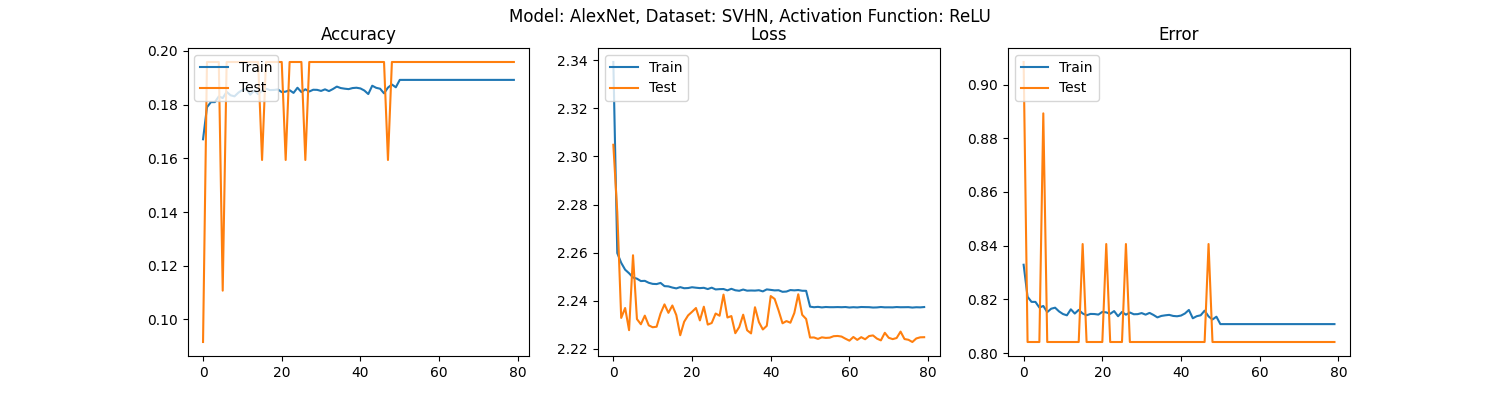
\includegraphics[width=400px,keepaspectratio]{AlexNet_SVHN_ReLU}
			\end{center}
			\begin{center}
				\centering
				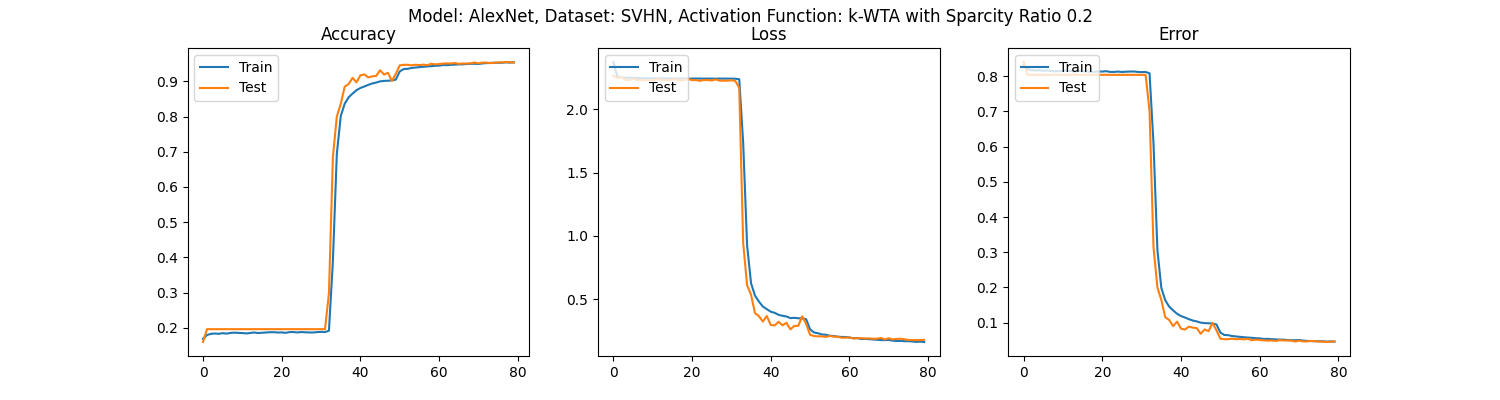
\includegraphics[width=400px,keepaspectratio]{AlexNet_SVHN_k-WTA_0.2.png}
			\end{center}
			\begin{center}
				\centering
				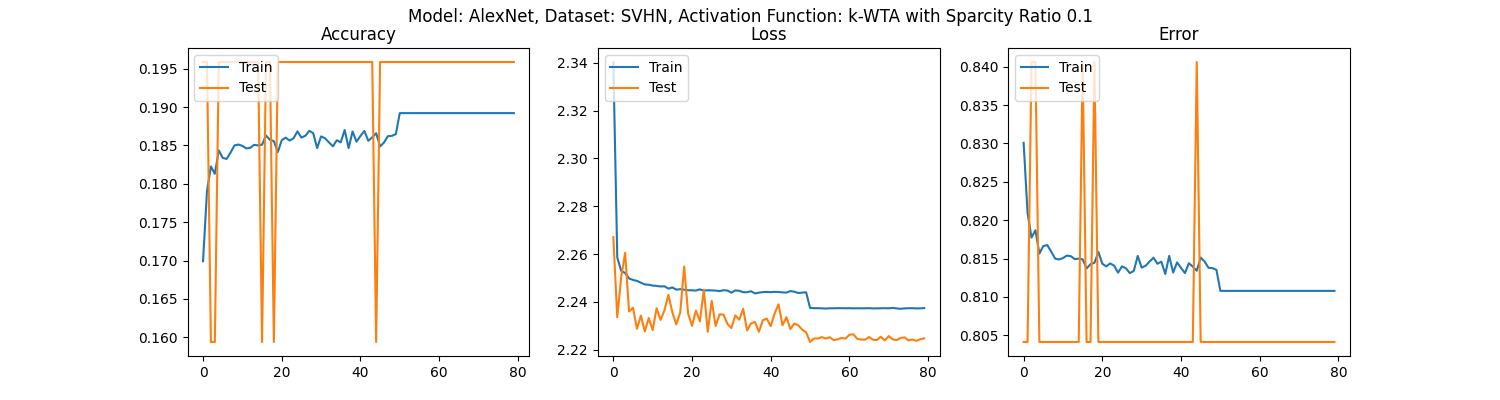
\includegraphics[width=400px,keepaspectratio]{AlexNet_SVHN_k-WTA_0.1.png}
			\end{center}
		
		\subsection{Pre-trained AlexNet on dataset SVHN}
			\begin{center}
				\centering
				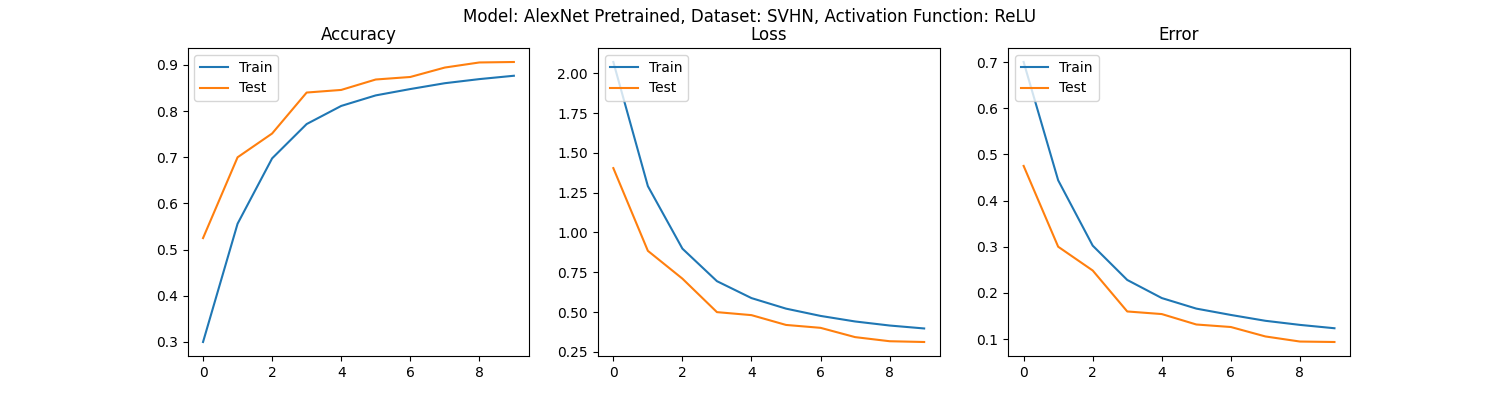
\includegraphics[width=400px,keepaspectratio]{AlexNet_SVHN_ReLU_Pretrained.png}
			\end{center}
			\begin{center}
				\centering
				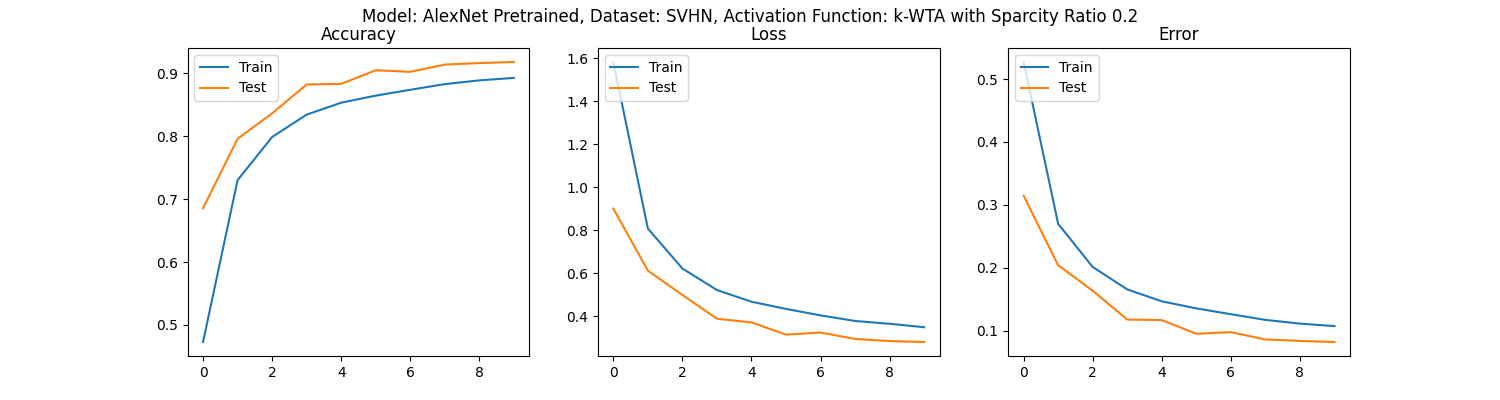
\includegraphics[width=400px,keepaspectratio]{AlexNet_SVHN_k-WTA_0.2_Pretrained.png}
			\end{center}
			\begin{center}
				\centering
				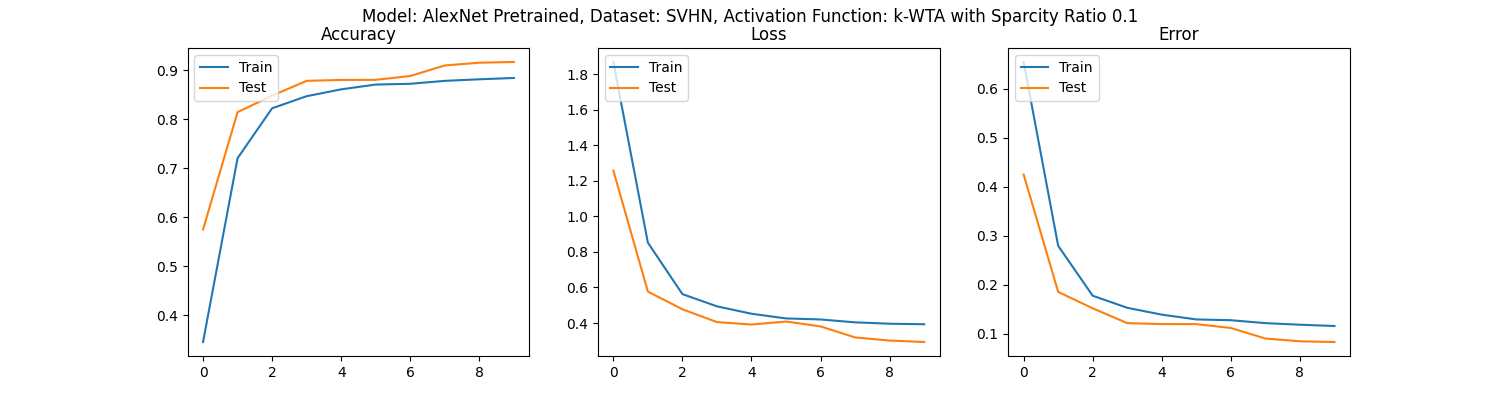
\includegraphics[width=400px,keepaspectratio]{AlexNet_SVHN_k-WTA_0.1_Pretrained.png}
			\end{center}
		
		\subsection{AlexNet on dataset CIFAR-10}
			\begin{center}
				\centering
				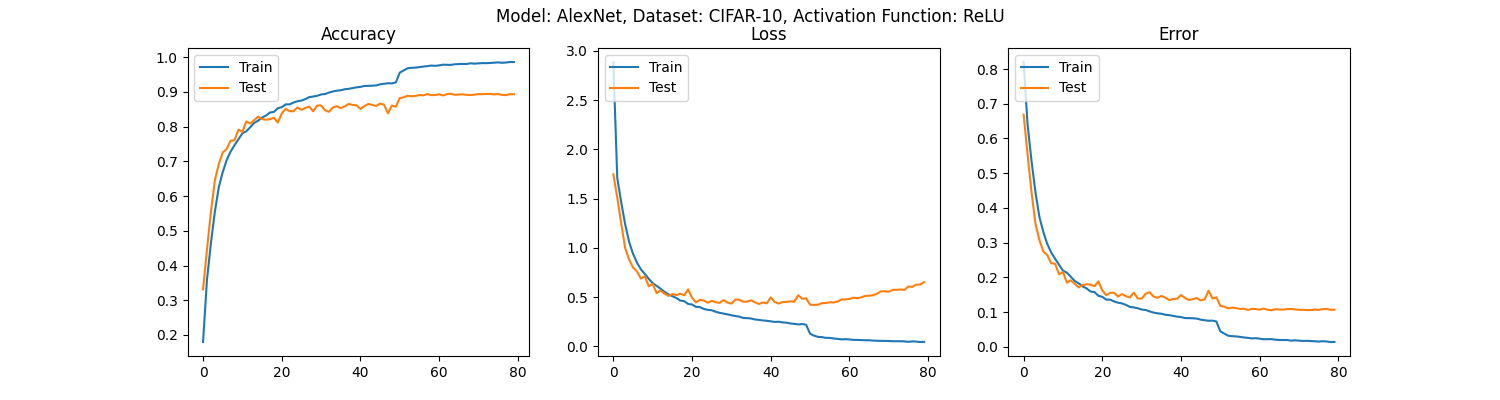
\includegraphics[width=400px,keepaspectratio]{AlexNet_CIFAR-10_ReLU.png}
			\end{center}
			\begin{center}
				\centering
				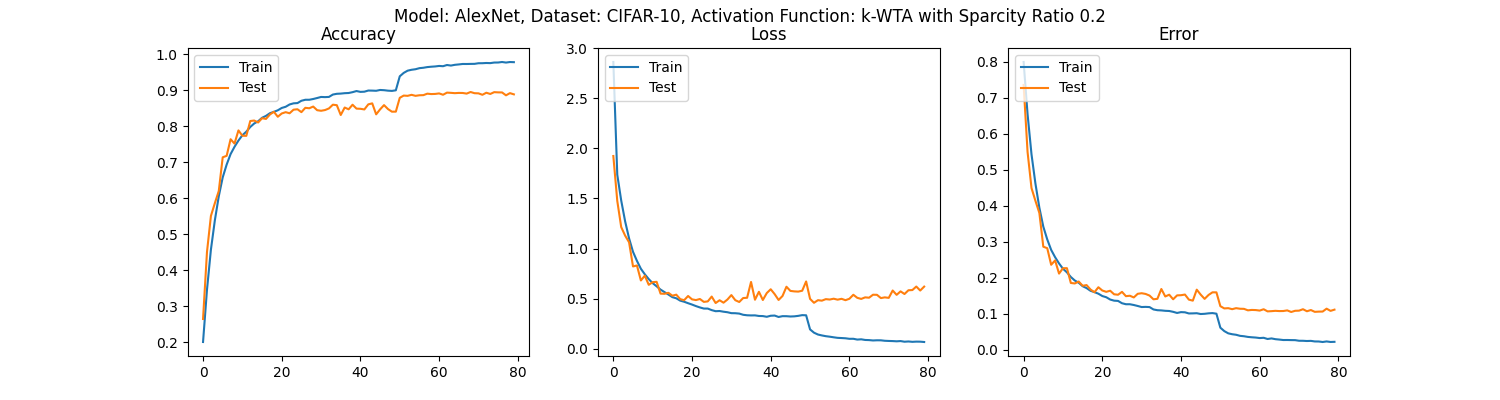
\includegraphics[width=400px,keepaspectratio]{AlexNet_CIFAR-10_k-WTA_0.2.png}
			\end{center}
			\begin{center}
				\centering
				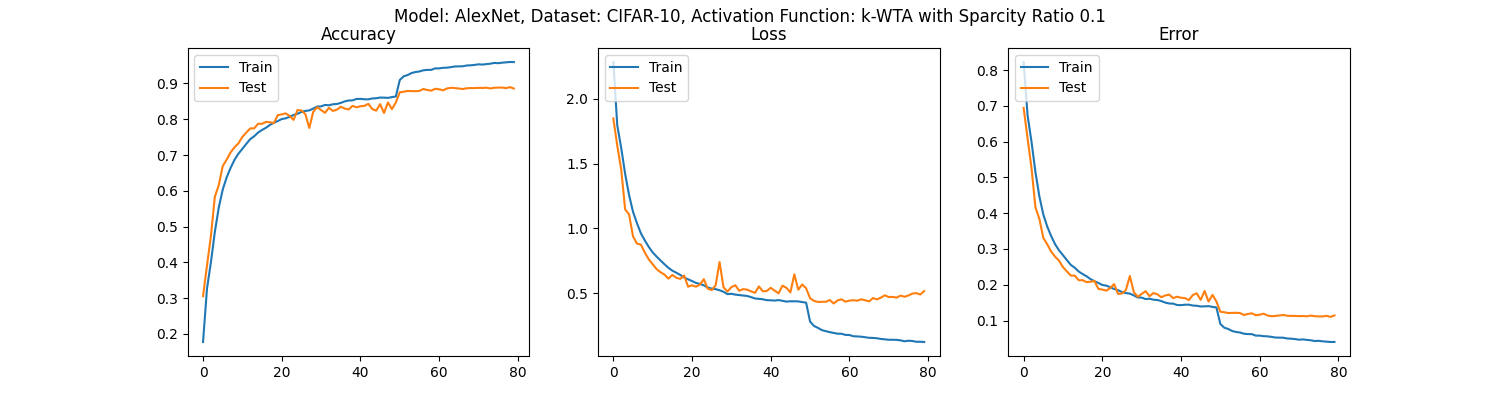
\includegraphics[width=400px,keepaspectratio]{AlexNet_CIFAR-10_k-WTA_0.1.png}
			\end{center}
		
		\subsection{Pre-trained AlexNet on dataset CIFAR-10}
			\begin{center}
				\centering
				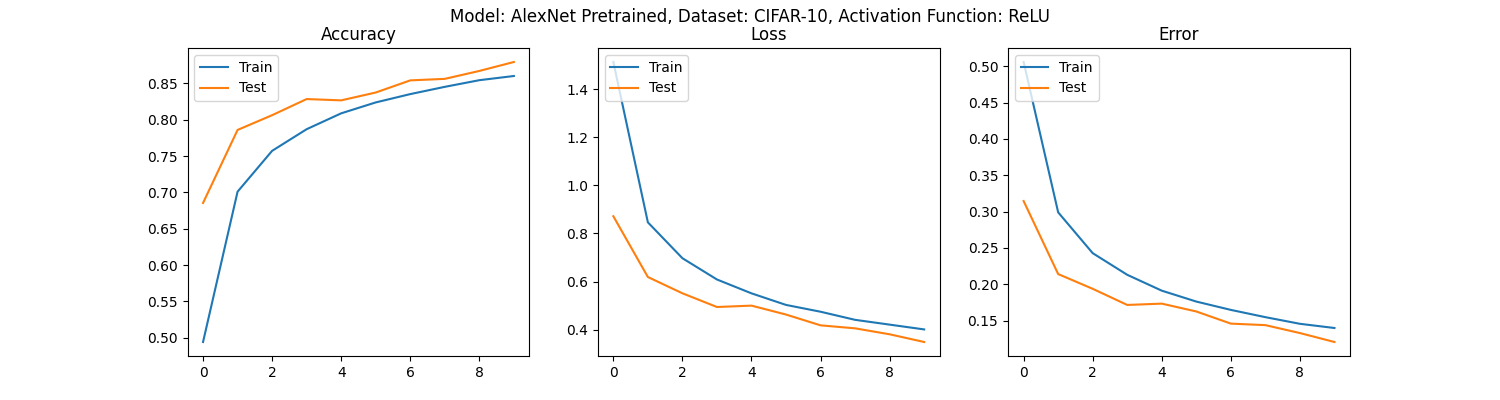
\includegraphics[width=400px,keepaspectratio]{AlexNet_CIFAR-10_ReLU_Pretrained.png}
			\end{center}
			\begin{center}
				\centering
				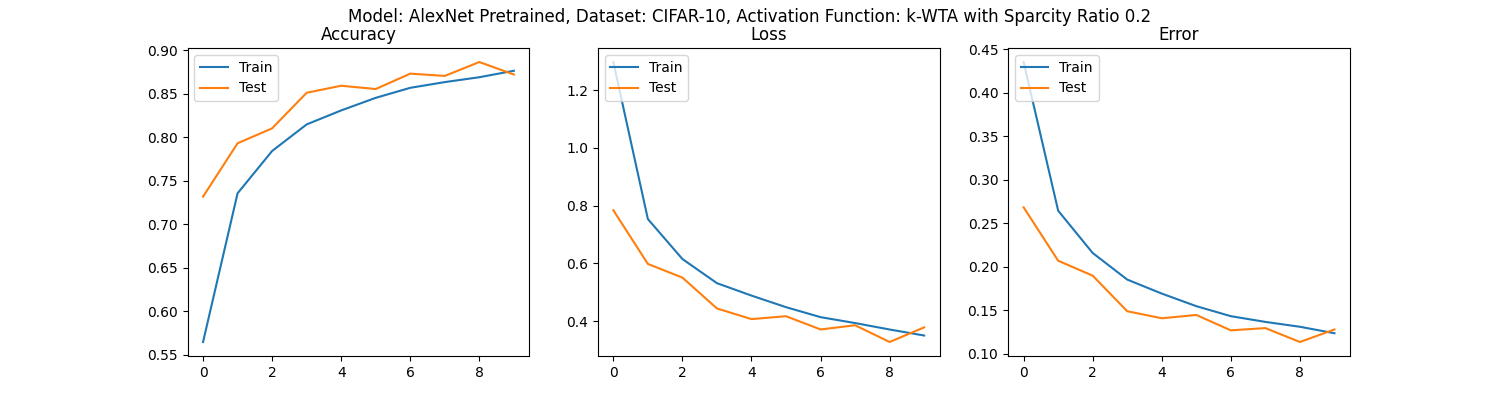
\includegraphics[width=400px,keepaspectratio]{AlexNet_CIFAR-10_k-WTA_0.2_Pretrained.png}
			\end{center}
			\begin{center}
				\centering
				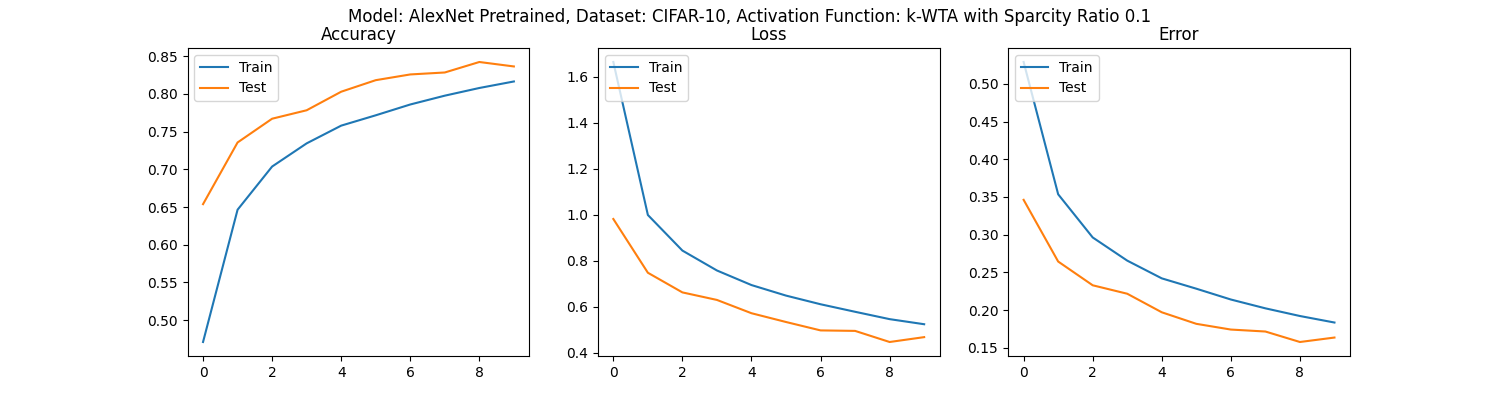
\includegraphics[width=400px,keepaspectratio]{AlexNet_CIFAR-10_k-WTA_0.1_Pretrained.png}
			\end{center}
		
		\subsection{ResNet18 on dataset SVHN}
			\begin{center}
				\centering
				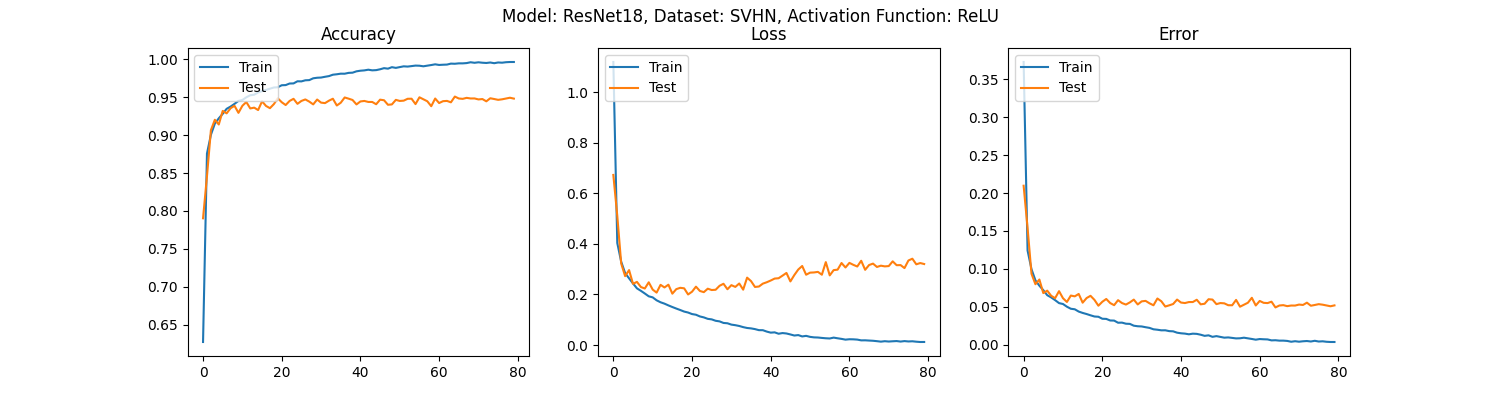
\includegraphics[width=400px,keepaspectratio]{ResNet18_SVHN_ReLU.png}
			\end{center}
			\begin{center}
				\centering
				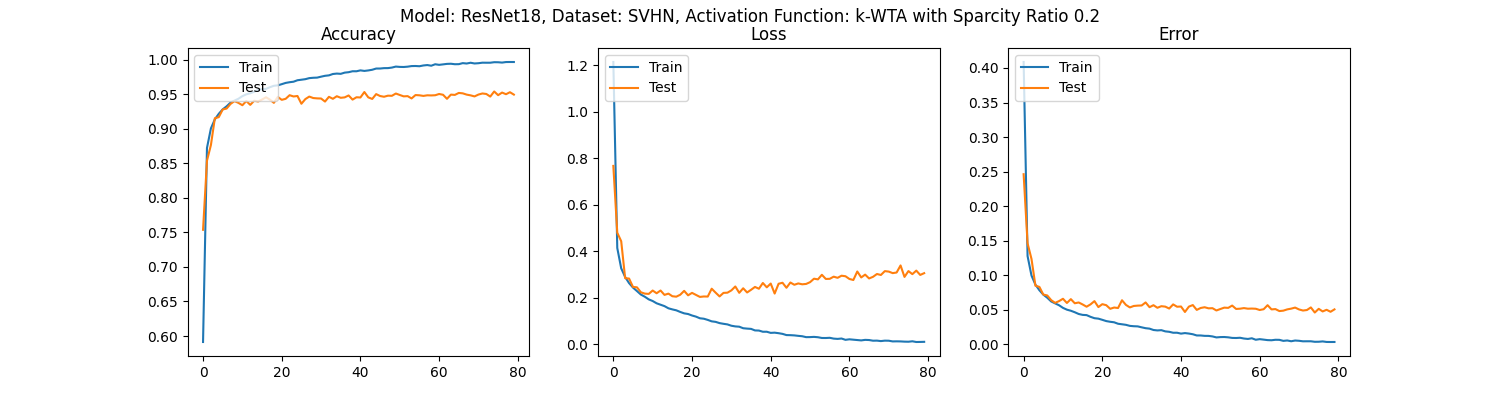
\includegraphics[width=400px,keepaspectratio]{ResNet18_SVHN_k-WTA_0.2.png}
			\end{center}
			\begin{center}
				\centering
				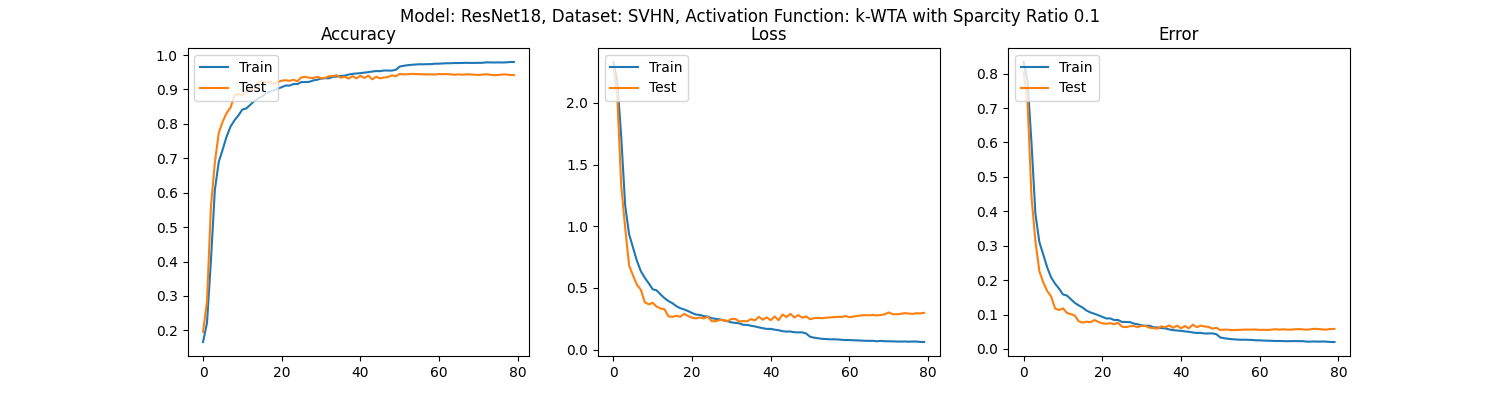
\includegraphics[width=400px,keepaspectratio]{ResNet18_SVHN_k-WTA_0.1.png}
			\end{center}
		
		\subsection{Pre-trained ResNet18 on dataset SVHN}
			\begin{center}
				\centering
				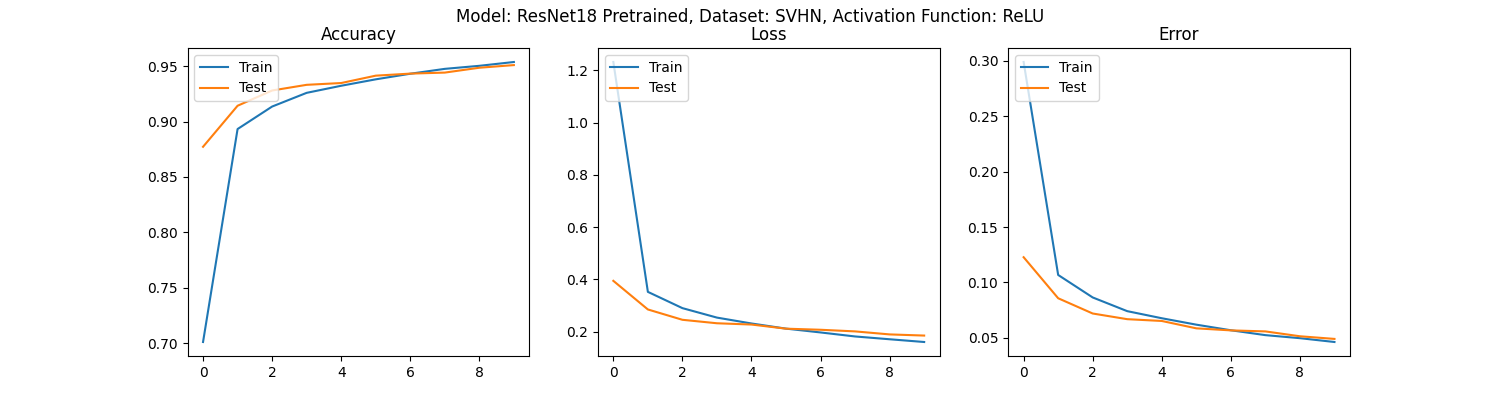
\includegraphics[width=400px,keepaspectratio]{ResNet18_SVHN_ReLU_Pretrained.png}
			\end{center}
			\begin{center}
				\centering
				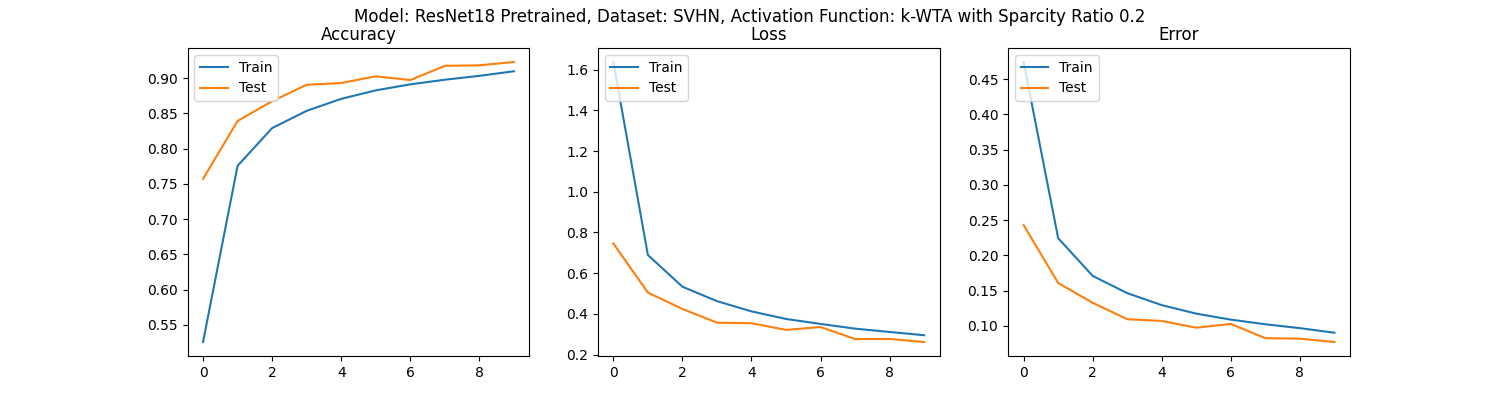
\includegraphics[width=400px,keepaspectratio]{ResNet18_SVHN_k-WTA_0.2_Pretrained.png}
			\end{center}
			\begin{center}
				\centering
				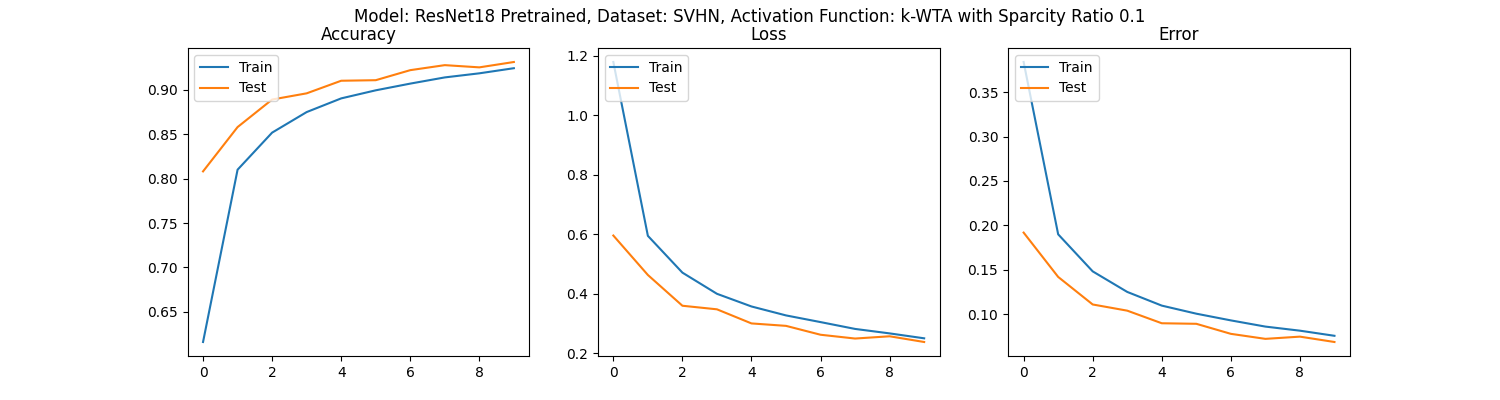
\includegraphics[width=400px,keepaspectratio]{ResNet18_SVHN_k-WTA_0.1_Pretrained.png}
			\end{center}
		
		\subsection{ResNet18 on dataset CIFAR-10}
			\begin{center}
				\centering
				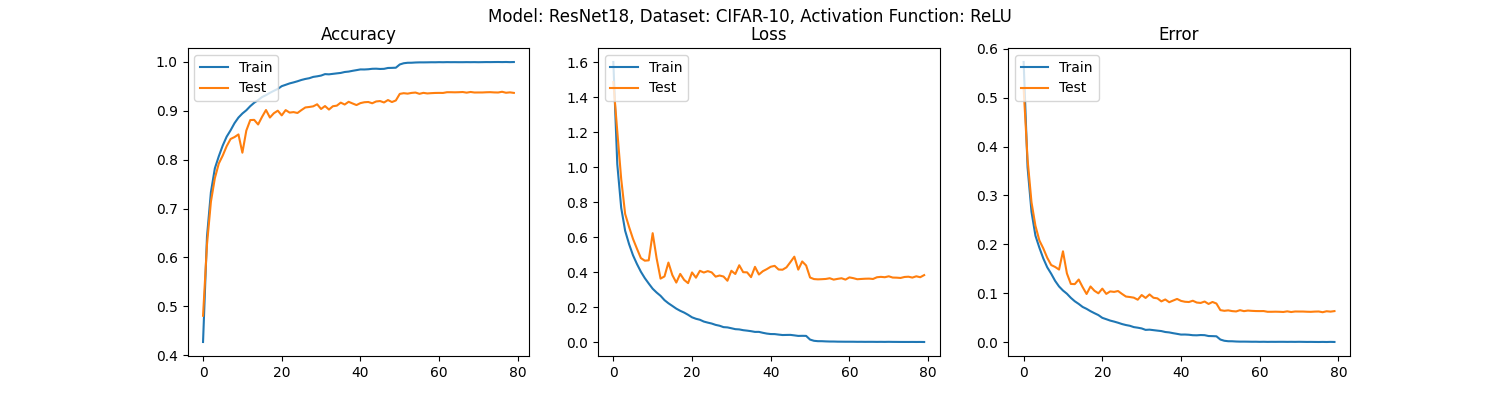
\includegraphics[width=400px,keepaspectratio]{ResNet18_CIFAR-10_ReLU.png}
			\end{center}
			\begin{center}
				\centering
				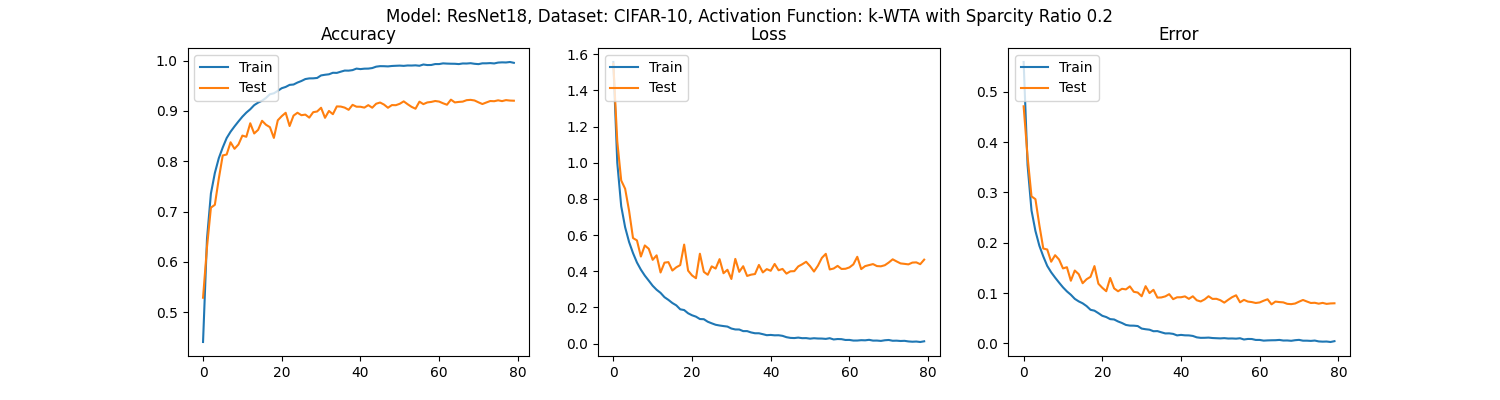
\includegraphics[width=400px,keepaspectratio]{ResNet18_CIFAR-10_k-WTA_0.2.png}
			\end{center}
			\begin{center}
				\centering
				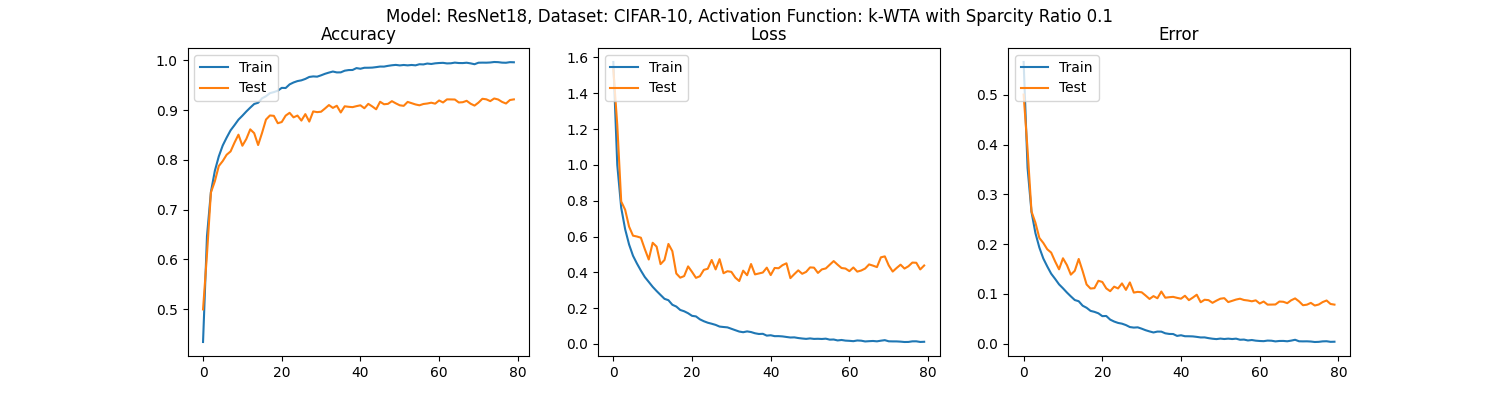
\includegraphics[width=400px,keepaspectratio]{ResNet18_CIFAR-10_k-WTA_0.1.png}
			\end{center}
		
		\subsection{Pre-trained ResNet18 on dataset CIFAR-10}
			\begin{center}
				\centering
				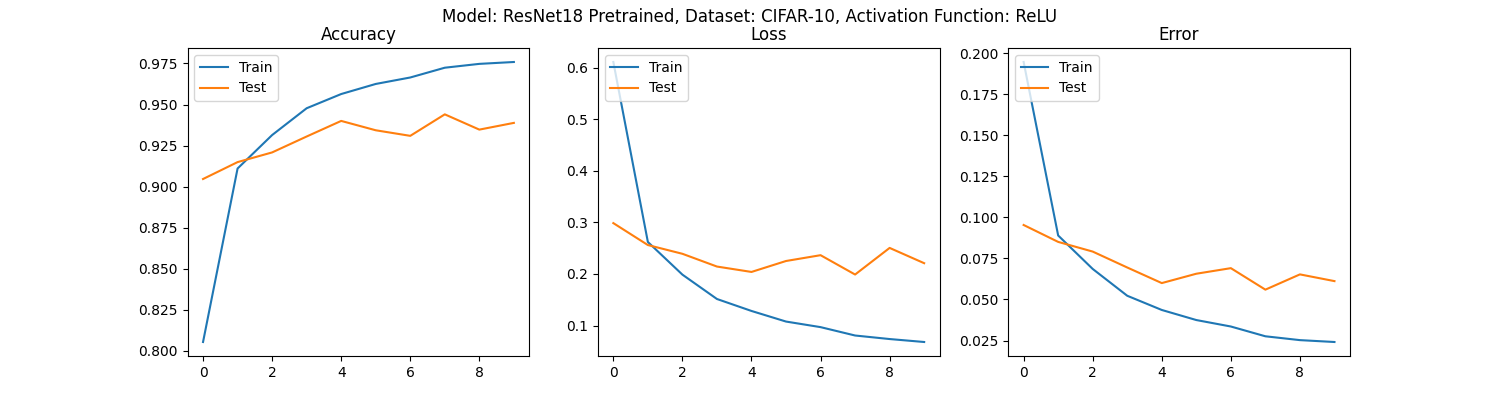
\includegraphics[width=400px,keepaspectratio]{ResNet18_CIFAR-10_ReLU_Pretrained.png}
			\end{center}
			\begin{center}
				\centering
				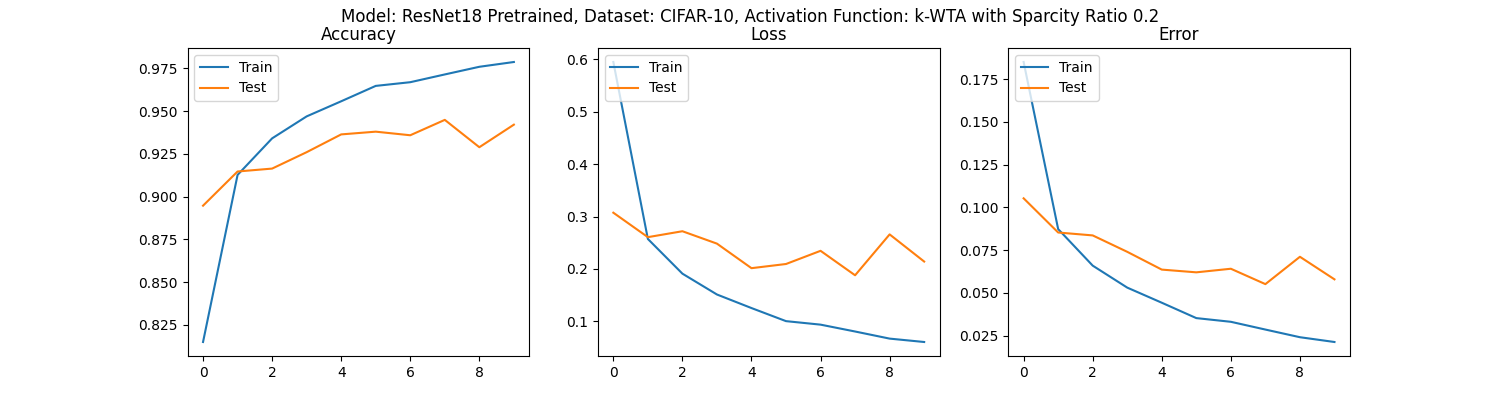
\includegraphics[width=400px,keepaspectratio]{ResNet18_CIFAR-10_k-WTA_0.2_Pretrained.png}
			\end{center}
			\begin{center}
				\centering
				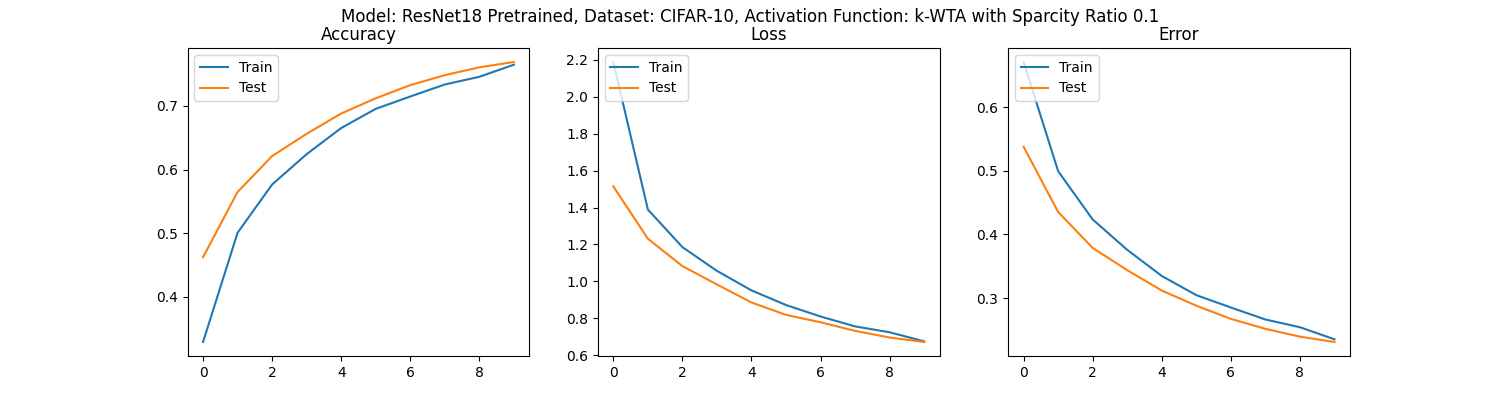
\includegraphics[width=400px,keepaspectratio]{ResNet18_CIFAR-10_k-WTA_0.1_Pretrained.png}
			\end{center}
		
		\bibliography{bibliography} 
		\bibliographystyle{ieeetr}
\end{document}